%%%%%%%%%%%%%%%%%%%%%%%%%%%%%%%%%%%%%%%%%
%
% (c) 2018 by Jennifer Laaser
%
% This work is licensed under the Creative Commons Attribution-NonCommercial-ShareAlike 4.0 International License. To view a copy of this license, visit http://creativecommons.org/licenses/by-nc-sa/4.0/ or send a letter to Creative Commons, PO Box 1866, Mountain View, CA 94042, USA.
%
% The current source for these materials is accessible on Github: https://github.com/jlaaser/pogil-polymers
%
%%%%%%%%%%%%%%%%%%%%%%%%%%%%%%%%%%%%%%%%%

\documentclass[book,instructor]{pogil}

%%%%%%%%%%%%%%%%% DOCUMENT INFORMATION %%%%%%%%%%%%%%%%%%%%%%%%

\author{Jennifer Laaser}
\institution{University of Pittsburgh}
\title{POGIL Polymers}
\subtitle{Guided-Inquiry Activities \\for Polymer Chemistry and Polymer Physics}
\date{\today}

\copyrightshort{
\includegraphics[width=0.1\textwidth]{by-nc-sa} J. Laaser 2018}
\copyrightfulltext{
	\textcopyright 2018 by Jennifer Laaser. \thetitle\ is made available under a Creative Commons Attribution-NonCommercial-ShareAlike 4.0 International License: \url{http://creativecommons.org/licenses/by-nc-sa/4.0/}

	The current source for these materials is accessible on Github:\\ 		\url{https://github.com/jlaaser/pogil-polymers}
}
\copyrightgraphic{by-nc-sa}


%%%%%%%%%%%%%%%%%%%%%%%%%%%%%%%%%%%%%%%%%%%%%%%%%%%%%%%%%%%%%%
%%%%%%%%%%%%%%%%%%%%%%%%%%%%%%%%%%%%%%%%%%%%%%%%%%%%%%%%%%%%%%

\begin{document}

\frontmatter
\pagestyle{empty}
\titlepage
\clearpage

\copyrightpage
\clearpage

\tableofcontents*
\clearpage

%\chapter{Introduction}

%\lipsum[1-12]

\mainmatter
\pagestyle{fancy}

\part{Introduction to Polymers}

	\chapter{From Molecules to Polymers}
		%%%%%%%%%%%%%%%%%%%%%%%%%%%%%%%%%%%%%%%%%
%
% (c) 2018 by Jennifer Laaser
%
% This work is licensed under the Creative Commons Attribution-NonCommercial-ShareAlike 4.0 International License. To view a copy of this license, visit http://creativecommons.org/licenses/by-nc-sa/4.0/ or send a letter to Creative Commons, PO Box 1866, Mountain View, CA 94042, USA.
%
% The current source for these materials is accessible on Github: https://github.com/jlaaser/pogil-polymers
%
%%%%%%%%%%%%%%%%%%%%%%%%%%%%%%%%%%%%%%%%%

\section{Activity Template}
\renewcommand{\figpath}{content/figs}

\textbf{Focus question:} Put a central question for the students to consider through this exercise here.

\subsection{Model 1:  ABC}

Here is the first model for students to consider

% to include images, put them in the folder specified by figpath and then use:
%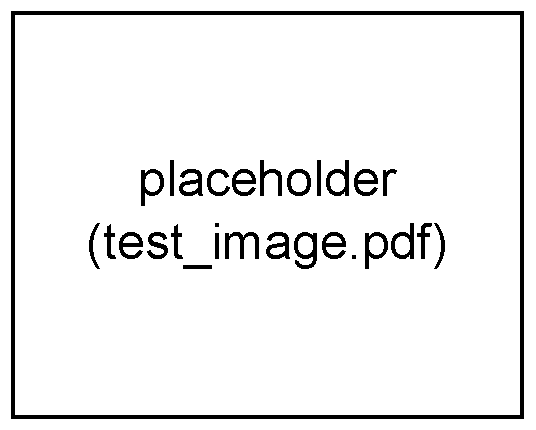
\includegraphics[width=0.8\textwidth]{\figpath/test_image.pdf}

\subsection{Critical Thinking Questions}

	\begin{enumerate}
		\item First question?
		\item Second question?
	\end{enumerate}

\subsection{Model 2: DEF}

\subsection{Critical Thinking Questions}

	\begin{enumerate}
		\item First question?
		\item Second question?
	\end{enumerate}

\subsection{Exercises}

	After class, \textbf{read} the following sections of your textbook:
	
	\begin{enumerate}
		\item First section
		\item Second section
	\end{enumerate}
	
	Then, do the following exercises:
	
	\begin{enumerate}
		\item First exercise
		\item Second exercise
	\end{enumerate}

\part{Polymer Chemistry}

	\chapter{Fundamentals of Polymer Chemistry}

	\chapter{Step-Growth Polymerizations}

	\chapter{Free-Radical Polymerization}

	\chapter{Controlled Polymerizations}

	\chapter{Copolymers}

\part{Polymer Physics}

	\chapter{Conformations of Polymer Chains}

	\chapter{Mechanical Properties of Polymers}

	\chapter{Phase Behavior of Polymers \& Their Solutions}

	\chapter{Thermal Properties of Polymers}


%\appendix

%\chapter{An Appendix Chapter}

%\lipsum[1-15]

\backmatter

\end{document}